\documentclass[border=6pt]{standalone}
\usepackage{amsmath}
\usepackage{tikz}
\usetikzlibrary{arrows.meta}
\begin{document}
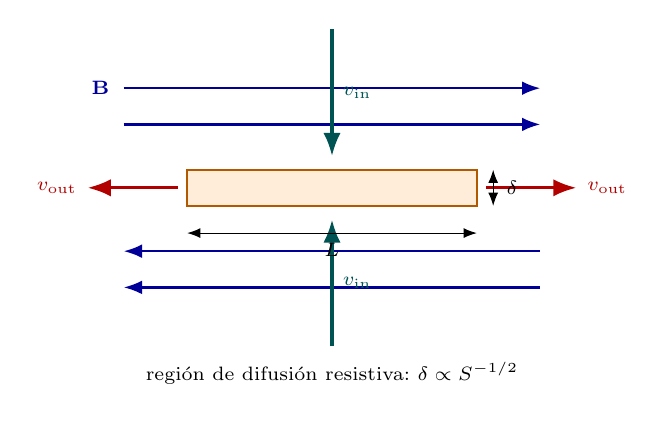
\begin{tikzpicture}[>=Latex,scale=1.15]

% region de difusion (lamina)
\fill[orange!15] (-1.6,-0.2) rectangle (1.6,0.2);
\draw[orange!70!black,thick] (-1.6,-0.2) rectangle (1.6,0.2);

% lineas de campo antiparalelas
\foreach \y in {0.7,1.1}{\draw[blue!60!black,thick,->] (-2.3,\y) -- (2.3,\y);}
\foreach \y in {-0.7,-1.1}{\draw[blue!60!black,thick,<-] (-2.3,\y) -- (2.3,\y);}
\node[blue!60!black,font=\scriptsize,anchor=east] at (-2.35,1.1) {$\mathbf B$};

% inflow (hacia la lamina)
\draw[->,teal!65!black,very thick] (0,1.75) -- (0,0.35) node[midway,right,font=\scriptsize]{$v_{\rm in}$};
\draw[->,teal!65!black,very thick] (0,-1.75) -- (0,-0.35) node[midway,right,font=\scriptsize]{$v_{\rm in}$};

% outflow (a lo largo de la lamina)
\draw[->,red!70!black,very thick] (1.7,0) -- (2.7,0) node[right,font=\scriptsize]{$v_{\rm out}$};
\draw[->,red!70!black,very thick] (-1.7,0) -- (-2.7,0) node[left,font=\scriptsize]{$v_{\rm out}$};

% dimensiones L y delta
\draw[<->] (-1.6,-0.5) -- (1.6,-0.5);
\node[font=\scriptsize,below] at (0,-0.5) {$L$};
\draw[<->] (1.78,-0.2) -- (1.78,0.2);
\node[font=\scriptsize,right] at (1.82,0) {$\delta$};

\node[font=\scriptsize,align=center] at (0,-2.05)
  {regi\'on de difusi\'on resistiva:\ $\delta \propto S^{-1/2}$};

\end{tikzpicture}
\end{document}
